% CHAPTER 1
\chapter{Introduction}

\section{Problem Definition}
To create a social platform for users to share location-sensitive content such as news, classifieds, and personal experiences. The central objective is to provide people with an open space to post any and all types of information pertaining to different real world locations. This information is posted and marked using virtual markers placeable at real world locations. These markers can be
viewed and navigated on connected apps and websites. A user can for example, point their
mobile cameras at a particular location to see any user submitted markers in that area. They
can also view them on maps or through shared links. This gives people a convenient
way to publish information publicly for anyone to find and view.
The process for creating a marker is as simple as visiting a location, selecting the content to post
and uploading it. Once a marker is placed, it can be discovered easily by anyone with a connected
app, through the methods discussed above.

\section{Motivation} 
The highlights of this project are its low cost and ease of use, as all users need to access
the service is a smartphone with GPS and internet connectivity. Therefore, such a service
might be readily accepted by the general public, leading to a significant change in the
way we share information.
We would also see a significant cut in pollution levels, as ad agencies turn to these
services instead of printing material that will litter the streets. The user driven curation
will curb bad advertising and promote healthy social trends.
As people are increasingly using their mobile phones for taking pictures and social
networking, this system provides them a way to use those activities for the betterment of
the community.
When it comes to information, visitors and tourists can now easily learn about various
places and their highlights. This will undoubtedly boost tourism and businesses in the
state.
Moreover, when people are more informed, they are less likely to fall for misinformation
and scams. They can make educated decisions in various spheres of life.
Thus, we would be seeing a much more informed and connected community which lead
to progress down the road.

\section{Existing System}
Google Maps is an existing system that implements several facets of our project and is widely popular among mobile applications. It presents users with detailed geographical information about any location they wish to look up. Moreover, it encourages user-added content including reviews, imagery and other media.
The key difference between our project and this existing system is that our platform favors more current and relevant information. We aim to create a social network where users share current events and subjective opinions rather than permanent and objective facts. Thus the nature of the content is dynamic and changes with time.
This allows users to learn about current happenings in a place instead of just information about the place. They can get familiar with the community and sentiment of people at that location, something that is not possible with the existing system. The addition of voting based discovery further improves the quality of information obtained.


\section{Scope of the Project}
1. An online social media platform for users to create, share and discover moments using virtual
markers.\\
2. Users can ``place'' digital content at real world locations, for others to find and view.\\
3. One can explore new locations from the comfort of their home by browsing through user
submitted content, before actually visiting those locations in person.\\
4. Works like a social news outlet, enabling people in a locality to discover and share
events happening there.\\
5. Businesses can use this platform to advertise their services to anyone visiting their area.\\
6. Different types of classifieds and announcements, can be posted for members of that
community to see.\\
7. A free community-centered initiative to develop public awareness and
relationships.

\chapter{Literature Survey}
\section{Mobile Location-Based Augmented Reality Applications for Urban Tourism Storytelling }

The implementation of context-aware mobile AR applications into tourism provides many benefits for the tourist experience. These apps can be used to enhance visitor learning in cultural heritage sites or advance the interaction between the visitor and tourist artifacts and often assume the form of games. Games have the power to create more engagement with the tourist destination through storytelling, playfulness and mobile learning.
\paragraph{}The demand for the fast creation of such games is increasing, with a large demand for changing new content to be delivered at a high pace. This requires new approaches for multimedia content creation beyond traditional field research. This includes using geo-location utilities and frameworks to gather points of interest (POI) or mining social networks in order to get collaborative feedback from other tourists or visitors.
\paragraph{}Smartphones, with the latest GPS-technology and built-in camera, enable players to use the real world as the playground and take gameplay outside into the real world. While the quantity and quality of mobile devices are increasing, mobile gaming attracts a wide range of user groups playing in different contexts. Recent advancements provide more people than ever access to hardware and new mobile game experiences. 
\paragraph{}Mobile gaming is lately evolving in travel and tourism opening new forms of creating enhanced experiences for tourists. Location-based, Augmented Reality (AR), Pervasive or Serious Games open the possibility to create deep, personalized and interactive experiences tourists are striving for by actively engaging the tourist with places and people throughout gameplay. This creates a deeper understanding and distinct experiences for the tourist with his immediate environment applying playful and gameful concepts. 

\subsection{Mobile AR and location-based storytelling in games }
Current multimedia systems in tourism enhance the reality with a digital layer of factual information about people, places and tourist relevant locations that would otherwise be invisible. The many AugmentedReality(AR)apps for travel and tourism such as Junaio1 and Wikitude2 curate much useful information to supply travellers with facts about the place visited. In many respects, these systems only loosely present information of tourist POIs as opposed to telling a whole story about places and engage the user into a narrative of the destination. Every place tells a story which can be told via new mobile technologies corresponding to the users current location via GPS and thus turning urban environments into a stage on which the narrative unfolds. Location-based storytelling is a powerful tool for tourism destinations to draw people in and make them understand the places they visit in a more interactive way than just presenting bare facts. 
\paragraph{}As with the further development of smartphones, creating engaging experiences with location-based mobile AR Games evolves from a niche to a wider audience. Mobile game design is currently experiencing a flourishing interest from game designers and game researchers. However, knowledge about game design for location-based mobile AR games in tourism are at an early stage as current research shows. Mobile game for tourists started with REXplorer, a pervasive game for the city of Regensburg, Germany with the aim to adduce the history of the city and give direction to the walking path through the city supported by audio-recorded material and in-game cha. Another example of mobile game-based learning has been conducted with Frequency 1550, a mobile city game placed in the medieval town of Amsterdam focusing on historical location-based storytelling. The location based mobile AR Game Time Warp is concerned about how form and content issues impact the players experience of presence. The game is anchored in the city of Cologne, Germany, drawing on famous characters and historical places of the city and exploring the boundaries between gaming and physical space.The study focuses on exploring the relationship between game design, the city context, narrative, embodiment and interaction. Outcomes revealed that game design needs to be strongly anchored either in a narrative or a location perspective in order to be successful. 
\paragraph{}Despite previous research on mobile location-based and AR games, little is known about how to design these games in a tourism context. This project explores the novel interdisciplinary topics of multimedia storytelling and game design in tourism to aim for creating engaging experiences for tourists. The use of location-based mobile AR games can intensify the way tourists interact with the physical and social environment and the way individual experiences are made.
\paragraph{}These location-based AR games still face the challenge of creating engaging experiences of the player with the environment although game designers scoop from a rich toolbox of game mechanics. Current games embrace elements of context awareness such as using urban landmarks for the gameplay to familiarize players with places or create interaction with the physical environment through interactive puzzles and quizzes. Another form of player engagement emerges in the social interaction among players and non-players liberated through role playing and engaging narratives.
\subsection{Conclusion}
The creation of game-based storytelling applications requires a well thought game design in order to identify the specific requirements of the tourists who behave like a player in the unfamiliar destination. Tourist destination management organizations (DMOs) need to know for which target audience prototyping has the advantage of producing large quantities of consumable information in a short period of time to retrieve user feedback in order to iteratively improve game design. It can have, however, not enough critical and curated information and detail brought by traditional story gathering techniques. 
\paragraph{}The current application features a full-fledged location-based game, using maps, an augmented reality utility and 3D game complement.The game was created for mobile platforms and follows a main story around the city of Porto and its wine production tradition. The game-base storytelling system has a well-designed strategy and all technologies were tested and implemented. The next stage will be the improvement of the user interface with additional user studies in order to deploy a final version, which will be used to create more engaging tourist experiences with the city of Porto.
\section{A concept of location-based social network marketing} 
\subsection{A model of location-based social network marketing }
A model of LSN marketing is conceptualized based on the insights from the focus group discussions. It is understood from the investigation that when facing a decision at a point of time and in a specific geographic area, consumers are exposed to marketing stimuli that include the venue characteristics, system rewards, competition-based social rewards, and connection-based social rewards. The consumption situations, consumer characteristics, and social network characteristics shape consumers’ perceptions of the stimuli, which would lead to a behavioral response (i.e., venue selection). At large, the scope of LSN marketing approach includes consumers’ decisions and mobility that spans over time and cover different geographic areas. In a travel context, for example, travelers face a series of decision-making processes that entail a combination of different venues (e.g., attractions and services) in different areas of the destination throughout the duration of the trip. Thus, LSN marketing for a tourism destination requires providing a combination of marketing stimuli that can be transformed into value maximizing strategies within space and over time (which can manifest in attraction selection and bundling,timing and duration, etc.). Likewise, the general users of LSN applications face similar decisions on a daily basis. Four square refresh the leader board everyweek, allowing users to re-strategize their competition and connection with others through consumption of places over time. These strategies may include an increase in overall patronage, which, as identified from the focus group discussions, can lead to loyalty and/or variety behavior.
\paragraph{}The model of LSN marketing is represented in Figure 1. As consumers are exposed to the marketing stimuli of various venues in
relevant areas through LSN applications (i.e., seen as desired consequences of strategies),they develop certain perceptions toward merchant rewards, competition-based rewards (which include application rewards and competition based social rewards), and connection-based rewards. Merchant reward typically includes a variety of monetary (e.g., price discount) and non-monetary (e.g., extra product) promotions at a venue that can be redeemed with a completion of certain tasks. Competition-based reward can be defined as the state of being recognized as the leader by members of consumers’ social network based on the accomplishment of application rewards. Connection-based reward is defined as the state of being well-connected with members of consumers’ social network as a result of interaction and communication. The higher the consumers perceive the rewards, the higher the tendency of actual behavior that may manifest in spatiotemporal strategies in the forms of loyalty behavior and/or variety behavior. 
\begin{figure}[h]
\center
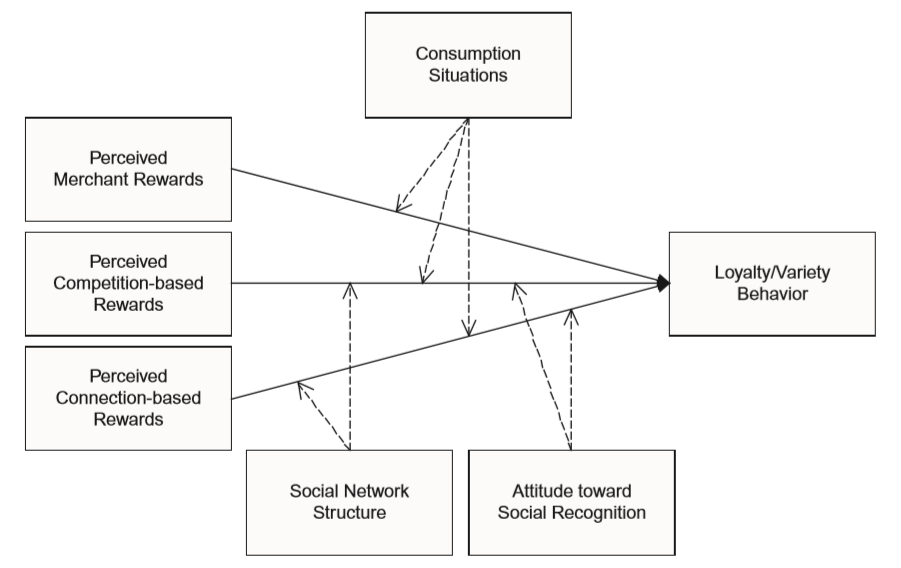
\includegraphics[scale=.8]{1.png}   
\caption{A Stimulus-Response Model of LSN Marketing }
\label{fig1}
\end{figure}
\paragraph{}Lastly, the intensity of communication and competition as well as consumers’ attitude toward social recognition influence the relationships between both the perceived competitionbased and connection-based rewards and actual behavior. Social network structure on LSN applications can be represented by measures of social network such as cohesion (i.e., the degree to which members are directly connected to each other) and/or density (i.e., the proportion of actual ties within a network relative to the total possible ties). The more cohesive and/or the denser the social network where consumers belong to, the more likely the perceived competition-based rewards (as well connection-based rewards) lead to actual behavior. It is noteworthy to emphasize that the social network serves as an environment for members to interact and connect with each other, directly and indirectly, causing social contagion to flourish. Additionally, individual’s attitude toward social recognition and status influences the relationships between the two perceived rewards and actual behavior. For consumers who exhibit a strong attitude toward social recognition, the more likely the perceived competitive-based rewards will lead to actual behavior, but the less likely the perceived connection-based rewards will.

\subsection{Conclusion}
As LSN applications on mobile phones become the new norm for people to experience what cities have to offer, it is of a great
importance to understand how to embrace the technology trend for marketing purposes, particularly in the context of tourism and hospitality businesses. The qualitative investigation utilizing focus group method identified valuable insights from users’ experiences, which were conceptualized into a stimulus-response model of LSN marketing. The key to LSN marketing is combining relevance and playfulness into a persuasive package that stimulates consumers’ loyalty and variety behavior and, in turn, shapes their mobility within the cities. The marketing stimuli identified in this investigation are the ability of the system to provide immediate rewards enabled by the technology features of LSN applications: context-awareness, social network, and social gaming. One of the perceived effective stimuli to change consumers’ behavior and mobility is the location-relevant merchant rewards made possible by the context aware system. Merchant rewards, which may include monetary and non-monetary promotions, are believed to be one of the driving forces of patronage behavior due to consumers’ value maximizing strategy. Competition-based rewards are the unique marketing stimuli facilitated by the combination of all three technology features of LSN applications. Using LSN applications, consumers gain personal enjoyment from receiving application rewards upon completion of certain tasks that allow them to compete with others in the social network. The playfulness of collecting points or unlocking badges by checking-in to local establishment is magnified by the status recognition from consumers’ social network. Competition-based rewards influence consumers to transform real life into a game, making mobility and experiences more playful and fun. The last marketing stimuli made available by LSN applications are the connection-based rewards, which are born from the combination of context-aware and social network features of the applications. LSN marketing persuades consumers to stay connected and broaden their social network by nurturing communication and interaction among members of the social network through instant updates and relevant recommendations.
\section{Augmented Reality in Mobile Devices}
Recent advancement in smartphone technology has fueled the popularity of Augmented Reality in mobile devices. We focus on the key technology required to develop a mobile Augmented Reality application. Discussing the existing problems . Finally, we provide an overview of the future 
scope and applications for Augmented Reality in mobile devices.
\subsection{Problems and Current Issues Existing in Mobile Augmented Reality }
 \textbf{Navigation and Tracking}: AR system utilize GPS for outdoor navigation because of 
its accuracy and high availability. But in urban environments the GPS reception and 
accuracy can deteriorate, where the GPS signal can be reflected and shadowed by the 
surrounding buildings. Magnetometers available in mobile devices can be used for the 
purpose of navigation and tracking, however, they can be affected by the local magnetic 
fields. 
\\\textbf{Content Management}: Many AR applications are limited in the way new content is 
be added to them. Programming skills are required for linking data sources to an existing 
system. Regular users should be able to add their own content with minimal technical 
effort. 
\\\textbf{Usability}: A user’s position and orientation is very important for an Augmented 
Reality application to behave as expected. Based on the location of the user, the digital 
6 
3D object is rendered into the real world. GPS sensors on smartphones have an accuracy 
of only 20 meters and the magnetometer compass orientation is only about 20 degrees. 
This will affect while calculating the field of view for the application, which will lead to 
digital objects and the real world not aligning with each other. 
    Although existing smartphones have high resolution camera they provide a limited 
field of view. Consequently, only a small portion of the user’s mobile field of view can 
be augmented. Identifying the Point of Interest to view the Augmented reality objects is a 
challenge the user must face. The user might have to rotate around while holding the 
device to locate the Point of Interest. 
 \\\textbf{Visualization}: The small display, brightness, resolution, contrast and field of view 
post as a challenge in Augmented Reality applications. The entire Augmented Reality 
application might not fit in the small display. The correct handling of the device is 
important for a realistic view if the virtual object is to rendered into the real world. 
  \\\textbf{Interaction Design}: The user interface and interaction of the user with an Augmented 
Reality application is still a problem, due to the small display of the mobile device. There 
are many challenges in achieving interaction of the user with the digital object. 
 \\\textbf{Hardware problems}: The hardware used should light weight and small so that it is 
easily portable. The problem with having a small device is its computational power. The 
battery life will be low and camera quality might not be good in most devices to display 
the augmented reality objects. 
  \\\textbf{Environmental issues}: The environment needs to be set up with markings to identify 
the locations for an AR application. 
\subsection{Key Technology}
\textbf{Tracking and Registration Technology}: Tracking and registration is the most 
challenging technology as it requires precise and accurate orientation tracking to align the 
virtual objects into the physical world. In an ideal scenario the tracking and registration 
technology should return the accurate camera position so that the rendered virtual objects 
can be placed in the correct position. When the camera position and orientation changes, 
the virtual object also should get superimposed on the changed position to make it 
perceive like it’s a real scene.
\\ There are two steps involved in the Tracking and Registration technology.
\begin{itemize}


\item Registration process: the virtual object should completely align itself to the 
correct position in the real world to achieve correct superposition.
\item Tracking process: When the observer position changes, the correct position 
between the virtual object and the real scene has to be reconstructed.  
\end{itemize}
 There are three types of tracking and registration methods 
 \begin{itemize}
 \item  Hardware-based tracking and registration method: This method mainly involves 
calculating the orientation and the spatial position of the object, based on the 
sensor data and signal sources acquired. 
\item Vision-based tracking and registration method: The data generated in the tracking 
phase, compares with stored data. Then it calculates the current orientation and 
position. It is fast simpler and has greater scalability. 
\item Hybrid tracking and registration method: It is the most promising method to deal 
with the indoor and outdoor environment difficulties. It is expensive and 
difficult to transplant.
\end{itemize}   
\textbf{Object Detection and Recognition Technology}: The main purpose of an Object 
detection and recognition technology is to discover the scene and find the target. It is 
divided into two parts. The first part is to emphasize on enhanced supplementary 
information to get a better perspective on the detection and classification. For example, in 
an Augmented Reality application after detecting the face, gender, name and age is 
displayed. The second part is image matching, the image features and corresponding 
11 
information are stored in the database on the MAR server. In an Augmented Reality 
system, the camera of the mobile device is used to capture the current image scene. 
Recognition technology is used to process the image, matches with respect to feature 
value. Finally displays the corresponding image in the camera field of view.  
    \\\textbf{Calibration}: Calibration technology utilizes the pixels of the image by the camera 
and restores the objects in real space. It is responsible for detecting the position and 
orientation and reporting the result data to the system. The calibration measured values 
are: the scope of vision, camera parameters, sensor offset, deformation and object 
localization. 
  \\\textbf{Model rendering}: The Model rendering technique is a process which utilizes 3D data 
to generate 2D images. The resulting image is usually stored in a frame buffer. OpenGL 
ES rendering technology is used in mobile devices to achieve rendering in Augmented 
Reality applications. It is a 2D/3D lightweight graphics library, specially designed for 
embedded and mobile devices.  
 \subsection{Conclusion}
 This paper gives a brief introduction about Mobile Augmented Reality. It defines what 
Mobile Augmented Reality [MAR] is and what are its challenges and concerns. It 
describes the generic framework required to develop an Augmented Reality application. 
We also discuss the existing Mobile Augmented Reality application available in different 
fields such as gaming, medical, military and advertisement and promotions. We have 
enlisted the different available Augmented Reality software platforms. 
  \paragraph{}  Cloud computing will play an important role in the future development of Augmented 
Reality applications. It will become a new trend and become a key role in developing 
MAR applications, since the cloud will undertake the heavy computational task, thereby 
saving energy and extending the battery life of the mobile device. Cloud services can 
operate as caches, decreasing the computational cost for both cloud services as well MAR 
applications. Mobile cloud computing seems as a promising new technology for 
promoting the development of MAR applications .
\paragraph{} 
    There seems to be a lot of future scope for Mobile Augmented Reality applications 
provided we eliminate all concerns and challenges. Privacy is one of the major concern 
for Augmented Reality. For example, pointing your phone to someone’s face which 
automatically pulls up their Facebook page could make some people weary. Even the 
user’s data such as the location of the user and personal information about the user 
present on the mobile device can be compromised while using an AR application. We 
hope more research on the topic will lead to the development of amazing Augmented 
Reality application without compromising user’s privacy and comfort. 
\section{An Emerging Study in Augmented Reality and Geographical Information System}
Geographic Information System (GIS) is rooted in intellectual practices, populated by data and powered by mathematical analysis. A survey conducted by Schuurman suggested that currently, the main use of GIS is for spatial analysis, predictive modelling, cartography and visualization. The SI Industry, also known as the GIS industry, is a rapidly growing industry. GIS maps the exact location and survey coordinates of an object in space to provide answer to queries using a computer system.
\paragraph{} Many popular applications like PokemonGO and Uber have great success with their brand as they have geo-based products. Users experience more engagement with the product when their location depends on it. This new trend has exposed the possibilities of geo-based apps and services as they have the most active users. Many of this geo-based apps have made a social impact with their users as they need to go out and move around to get the most out of the app. It has also allowed the users to be more active physically which is a great initiative to be more connected with the world.
\paragraph{} As these geo-based apps gain popularity among users, lawmakers are eyeing geolocation apps as there are many privacy concerns have arisen regarding user tracking. Today, GPS location-aware smart phones and other devices collect enormous amounts of data about where people go and what they do. This information can be aggregated with other information to determine ‘who they are’ with precision and accuracy.
\paragraph{} As geolocation is becoming an important component of daily lives (Ex. Navigation devices), geolocation will face a raft of new regulations. To avoid leaking consumer data and protecting their privacy, greater protection of the data should be accounted for.
\paragraph{} This independent has helped the understanding of why geo-based systems are so popular nowadays and their usefulness for users. With the end product being a location based system which may be used for building navigation or even open house navigation/information for universities, this system could greatly benefit communities that need geo-based systems to help people learn the advantages and possibilities of having location as a main factor for an application.
\subsection{Methodology}
Typically, geolocation apps do two things: They report your location to other users, and they associate real-world locations (such as restaurants and events) to your location. Geolocation apps that run on mobile devices provide a richer experience than those that run on desktop PCs because the relevant data you send and receive changes as your location changes.
\paragraph{} To become familiar with the topic of GIS and AR, some resources that have greatly improved the skills needed for this project are the Google Maps API. To store objects like places, buildings, points, etc., Google Maps greatly helps with understanding how these objects are made and stored in the database schema.
\paragraph{} Some products that are related to this specific study is Foursquare. With this geolocation service, users are able to check in to cafés, bars, restaurants, and pretty much anyplace. Aside from the social impact of checking in to a place when you’re actually there, it empowers users to collect stamps/badges to track progress of places visited, and overall keeping the consumer engaged with the application.
\paragraph{} Hackathon participation has also increased knowledge of the topic as it has allowed to quickly iterate concepts to proof the potential of geolocation applications. Hackathon experience has greatly increased quick adaptation of new concepts such as GIS/AR, and database schemas for geographical information which are used in this study. 
 
\subsection{Conclusion}
As geo-based applications are becoming popular and getting more exposure, a study like this shows how geolocation can be used to make systems that allow more immersive experiences with the surroundings around a person. This study has helped understand how geolocation works and how we can use places like buildings and build entities on top on them. As a student, this study greatly helps the understanding of how to build a geolocation service for consumers. As this is a current work in progress, the expectations for Spring semester is to fully bring this project to life and test a pilot with the Open House events to provide prospective students with an immersive experience of the campus.
 

\chapter{System Design and Analysis}
The proposed system is an application that runs on the user's phone. It communicates with an online back-end service that provides markers and other requested information to the client. The system must be responsive and offer seamless updating of content to ensure a smooth experience.\\\\
Steps of operation:\\
i.	Users visit a real-world location and turn on their mobile GPS\\
ii.	The connected app searches for and displays markers nearby, using AR or maps\\
iii.	The user can explore these markers or create a new one at their location\\
iv.	Markers can also have visibility settings to decide who can see it and from how far\\
v.	Markers can also have their content up-voted or down-voted by visitors\\
\begin{figure}[h]
\center
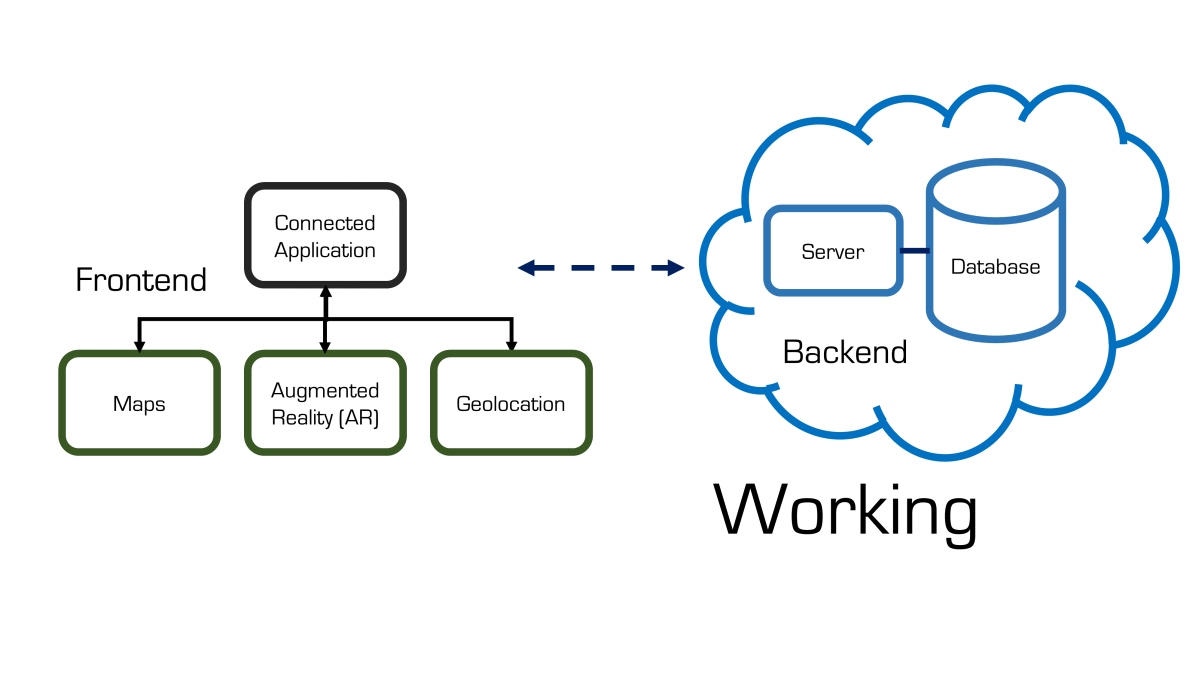
\includegraphics[scale=1.0]{sys_design.png}   
\caption{Marqur System Design }
\label{fig1}
\end{figure}
\pagebreak\\
\section{System Specification}
\begin{itemize}
\item The application requires an Android device with an internet connection in order to function.
\item A camera, GPS and compass(magnetometer sensor) are essential for the AR and nearby discovery features to work.
\item A minimum Android version of 4.1 (Jelly Bean) is required to run the app.
\item The cloud back-end will be hosted using Google's Firebase - A platform for developing and hosting mobile application back-ends.
\end{itemize}
  

\chapter{Conclusion and Future Work}
The proposed system gives users a place to share location based news and updates while promoting discussions and close-knit communities around the world. It gives users a general awareness of their surroundings and helps them scope out places before visiting them in person. In this way, it empowers people by giving them useful information on the go.
In the future, we plan on extending this project with monetization strategies such as advertisements and promoted posts. We also plan on integration of our project with existing internet services so the users may enjoy a connected experience.  


